\documentclass[a4paper,12pt]{article}

% Paquetes básicos
\usepackage[utf8]{inputenc}
\usepackage[T1]{fontenc}
\usepackage[spanish]{babel}
\usepackage{graphicx}
\usepackage{xcolor}
\usepackage{lipsum}
\usepackage{geometry}
\geometry{top=3cm, bottom=3cm, left=2.5cm, right=2.5cm}

% Paquetes para diseño
\usepackage{titlesec}
\usepackage{fancyhdr}
\usepackage{amsmath}
\usepackage{amssymb}
\usepackage{hyperref}

% Paquetes para el entorno lstlisting
\usepackage{listings}
\usepackage{inconsolata}

% Paquete para fondo
\usepackage{background}
\usepackage{pdfpages}

% Configuración de lstlisting
\lstset{
    language=Python,
    basicstyle=\ttfamily\small,
    keywordstyle=\color{blue}\bfseries,
    stringstyle=\color{teal},
    commentstyle=\color{gray}\itshape,
    numbers=left,
    numberstyle=\tiny\color{gray},
    backgroundcolor=\color{black!5},
    frame=single,
    rulecolor=\color{black!50},
    breaklines=true,
    captionpos=b,
    showstringspaces=false
}

% Configuración de título
\titleformat{\section}{\normalfont\Large\bfseries}{\thesection}{1em}{}

% Información del documento
\title{
    \vspace{-2cm}
    
\includegraphics[width=0.3\textwidth]{images/fccee.jpg} \\ % Cambia el logo si es necesario
    \LARGE Ingeniería Informática + ADE\\
    \large Universidad de Granada (UGR)\\[1cm]
}
\author{\textbf{Autor:} Ismael Sallami Moreno}
\date{\textbf{Asignatura:} Resúmenes de Contabilidad Financiera I}

% Configuración del fondo
\backgroundsetup{
    scale=1,
    color=black,
    opacity=0.2,
    angle=0,
    position=current page.south,
    vshift=0pt,
    hshift=0pt,
    contents={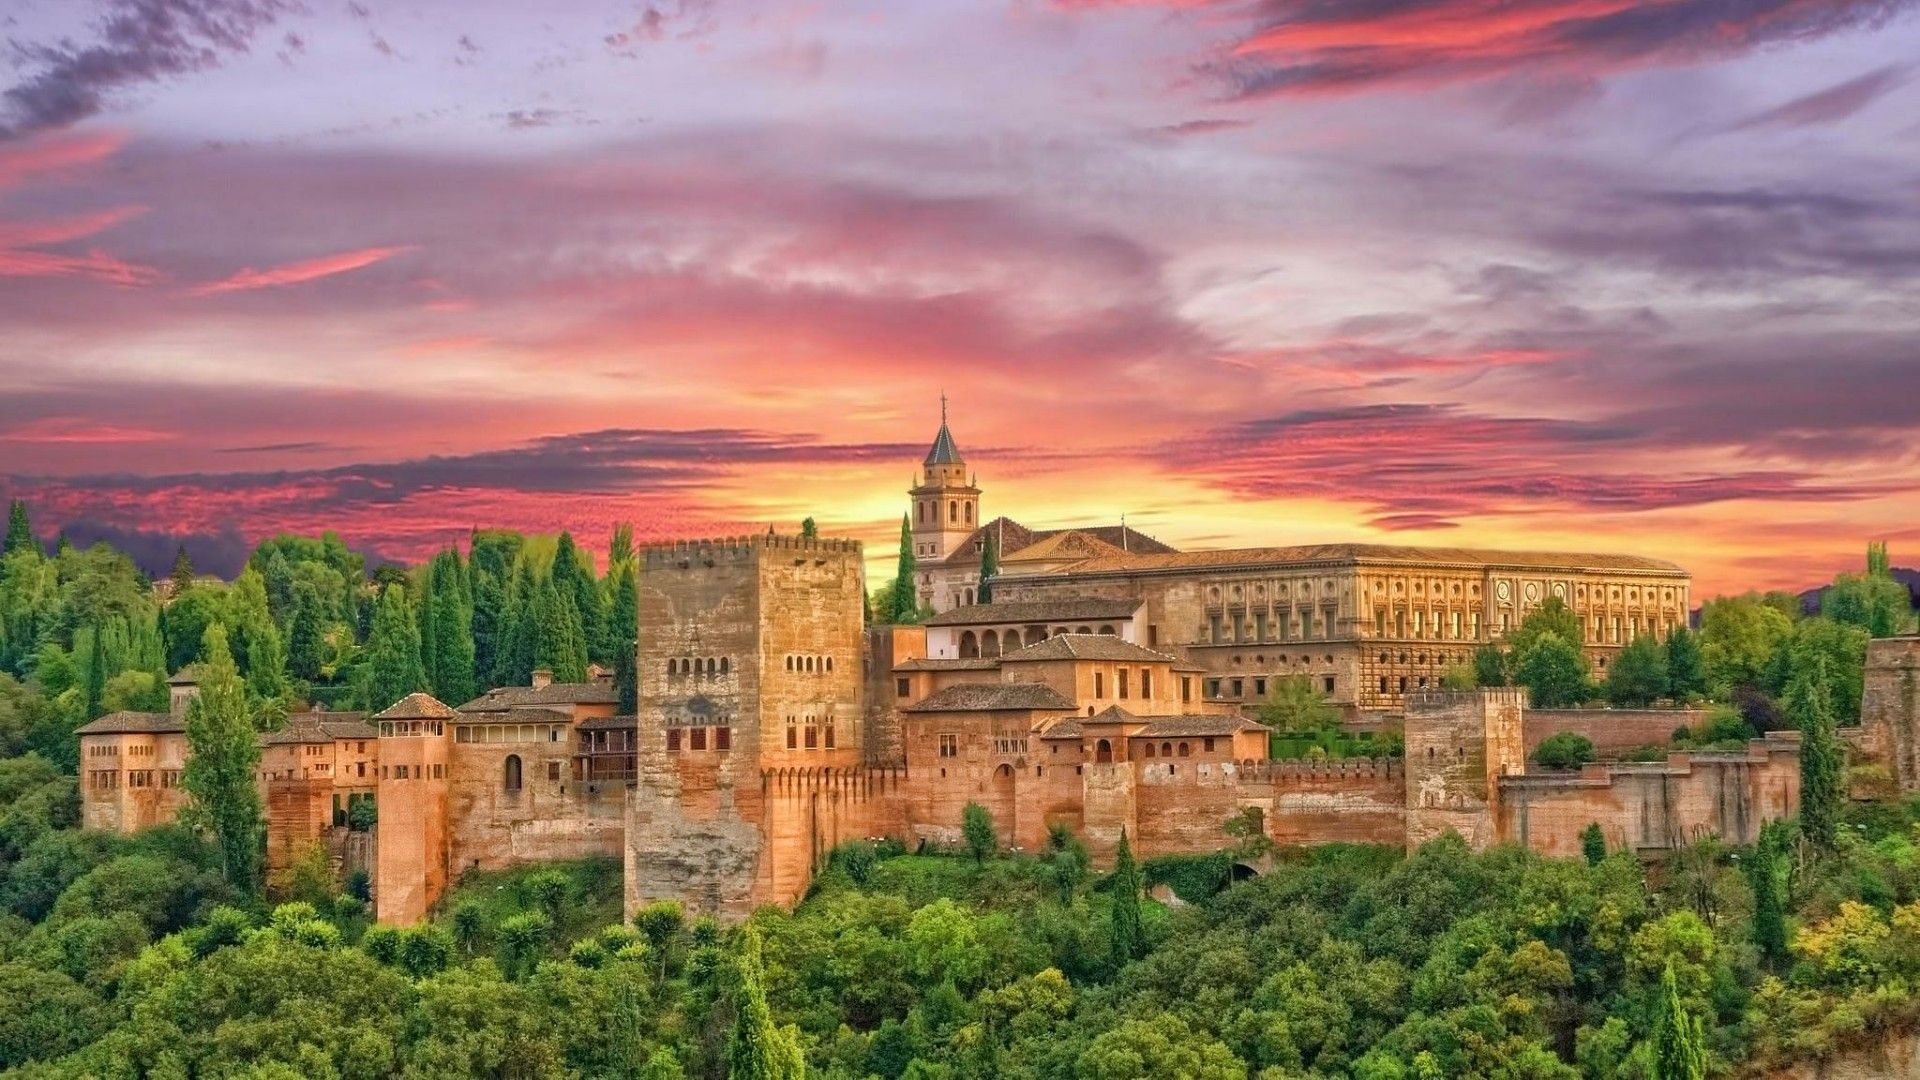
\includegraphics[width=\paperwidth,height=\paperheight,keepaspectratio]{images/granada.jpg}}
}

% Inicio del documento
\begin{document}

% Portada
\maketitle
\thispagestyle{empty}

\begin{center}
    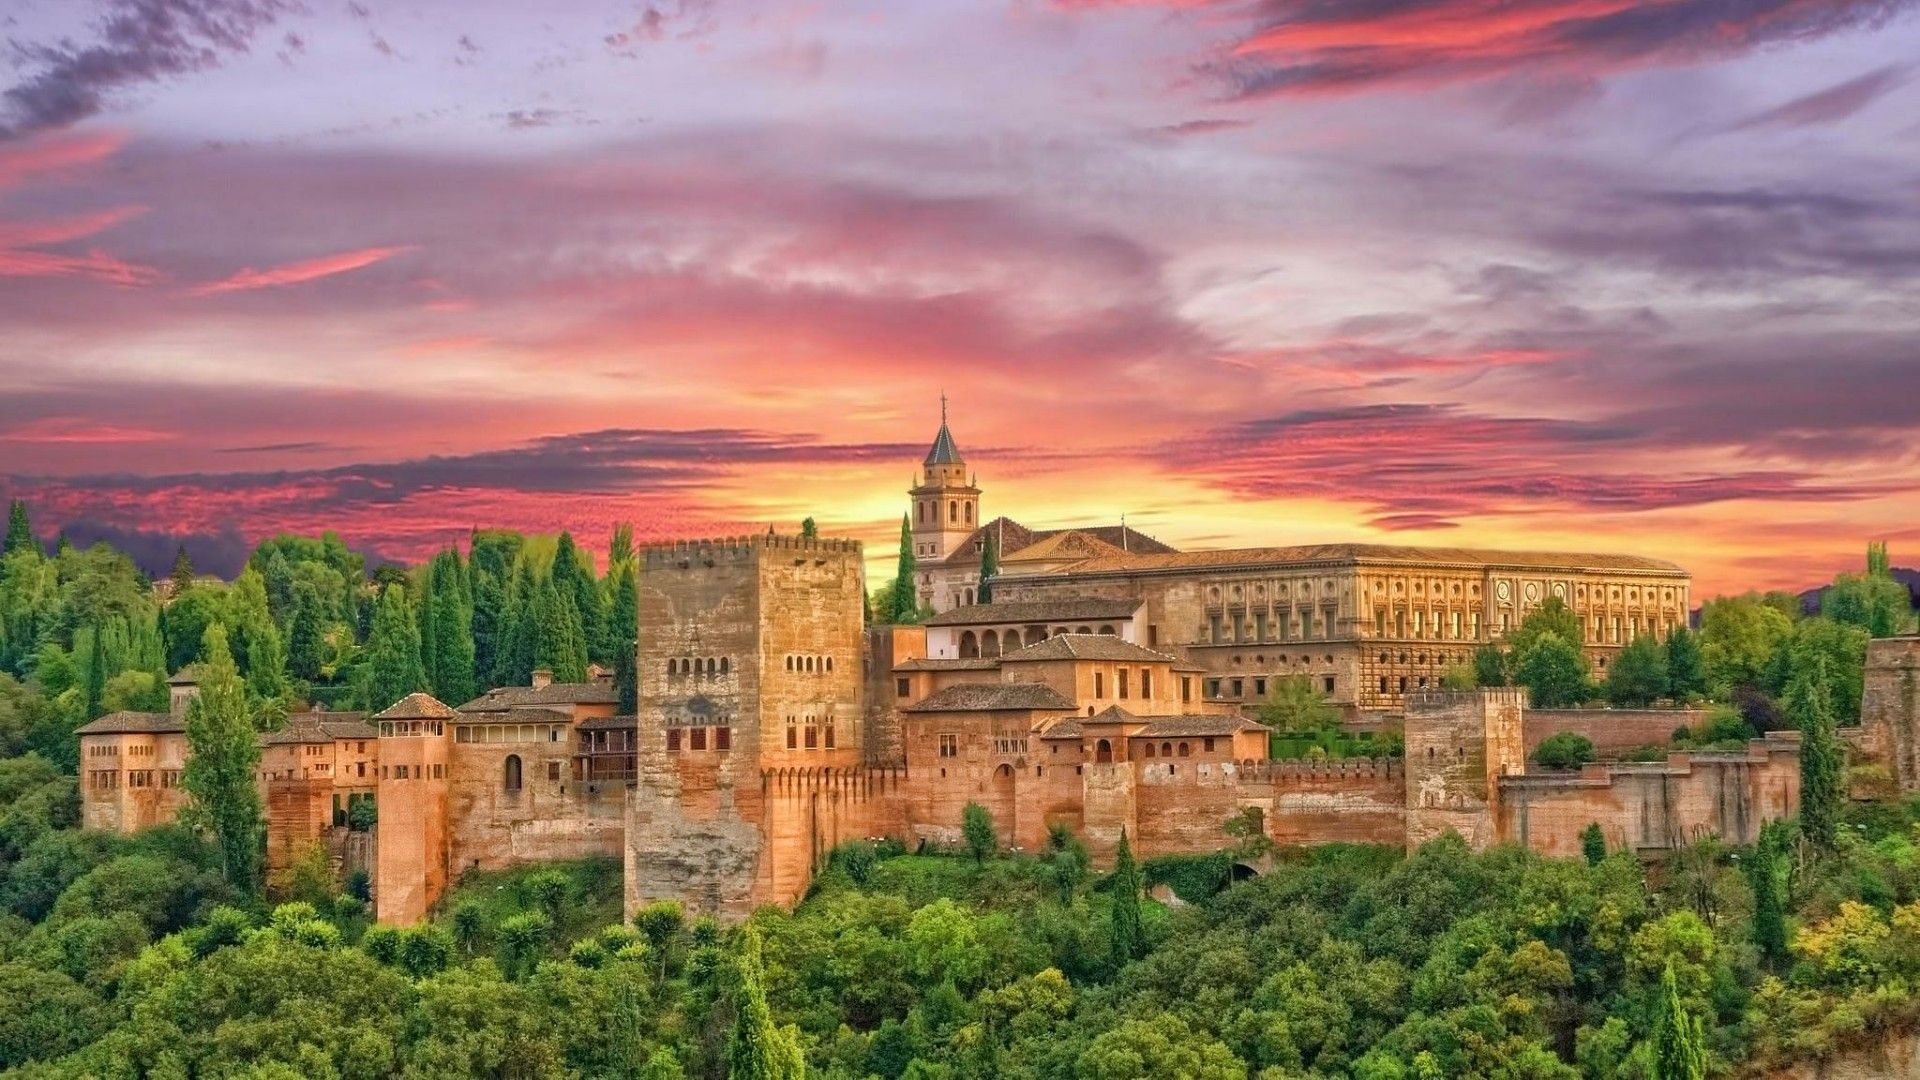
\includegraphics[width=\textwidth,height=0.4\textheight,keepaspectratio]{images/granada.jpg} \\ % Añade tu imagen de fondo
    \vfill
\end{center}

\newpage

% Índice (opcional)
\tableofcontents
\newpage

% Secciones
\section{Tema 1}
%\addcontentsline{toc}{section}{Tema 1}
\begin{center}
    \vspace*{2cm}
    \vspace*{1cm}
    \Large\textit{Resumen y Conceptos Clave}
    \vspace*{2cm}
\end{center}
\newpage
\includepdf[pages=2-,link,linkname=tema1]{../Tema1/FCCEE/build/Resument1.pdf}

\section{Tema 2}
%\addcontentsline{toc}{section}{Tema 2}
\begin{center}
    \vspace*{2cm}
    \vspace*{1cm}
    \Large\textit{Resumen y Conceptos Clave}
    \vspace*{2cm}
\end{center}
\newpage
\includepdf[pages=2-,link]{../Tema2/FCCEE/build/Resument2.pdf}

% \section{Tema 3}
% %\addcontentsline{toc}{section}{Tema 3}
% \begin{center}
%     \vspace*{2cm}
%     \vspace*{1cm}
%     \Large\textit{Resumen y Conceptos Clave}
%     \vspace*{2cm}
% \end{center}
% \newpage
% \includepdf[pages=2-,link]{../Tema3/FCCEE/build/Resument3.pdf}

\section{Tema 4}
%\addcontentsline{toc}{section}{Tema 4}
\begin{center}
    \vspace*{2cm}
    \vspace*{1cm}
    \Large\textit{Resumen y Conceptos Clave}
    \vspace*{2cm}
\end{center}
\newpage
\includepdf[pages=2-,link]{../Tema4/FCCEE/build/Resument4.pdf}

\section{Tema 5}
%\addcontentsline{toc}{section}{Tema 5}
\begin{center}
    \vspace*{2cm}
    \vspace*{1cm}
    \Large\textit{Resumen y Conceptos Clave}
    \vspace*{2cm}
\end{center}
\newpage
\includepdf[pages=2-,link]{../Tema5/FCCEE/build/Resument5.pdf}

\section{Tema 6}
%\addcontentsline{toc}{section}{Tema 6}
\begin{center}
    \vspace*{2cm}
    \vspace*{1cm}
    \Large\textit{Resumen y Conceptos Clave}
    \vspace*{2cm}
\end{center}
\newpage
\includepdf[pages=2-,link]{../Tema6/FCCEE/build/Resument6.pdf}

\end{document}
